\documentclass[english]{article}
\usepackage[T1]{fontenc}
\usepackage[latin9]{inputenc}
\usepackage{babel}
\usepackage{graphicx}
\usepackage{subfigure}
\usepackage{float}
\setlength{\parindent}{0pt}
\usepackage{amsmath}


\begin{document}

\title{Lab 1: Infrared Imaging\\ -------------------------------- \\ \Large Sensors and Digitization}
\author{ \ Armine Vardazaryan, Songyou Peng \\ arminevardazaryan@gmail.com, psy920710@gmail.com}
\date{26th November 2015}

\maketitle

\section{Introduction}
In this laboratory work we studied an infrared imaging system and its properties. 
We used it to measure the temperature of objects. \\
The system comprised a computer and an infrared camera Cedip SC7000 with its software Altair.\\
\section{Defect detection using IR camera}
In this section, after studying how to use the software and creating a project and connecting the camera, we use it to find the hot transistor on a circuit.\\

\begin{figure}[H]
	\centering
	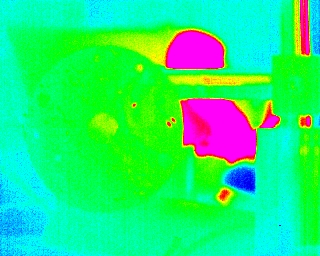
\includegraphics[width=0.3\linewidth]{Pictures/circuit_cold001.JPG}
	\caption{The IR image of the circuit with power off}
	\label{fig:one}
\end{figure}
In the image above the vague shape of the circuit can be seen in green. 
Because the circuit in the image is not connected to the power supply, it can be observed that the temperature appears to be uniform all around the surface of the circuit.\\
However, when the circuit is turned on, we see a region change its color.\\
\begin{figure}[H]
	\centering
	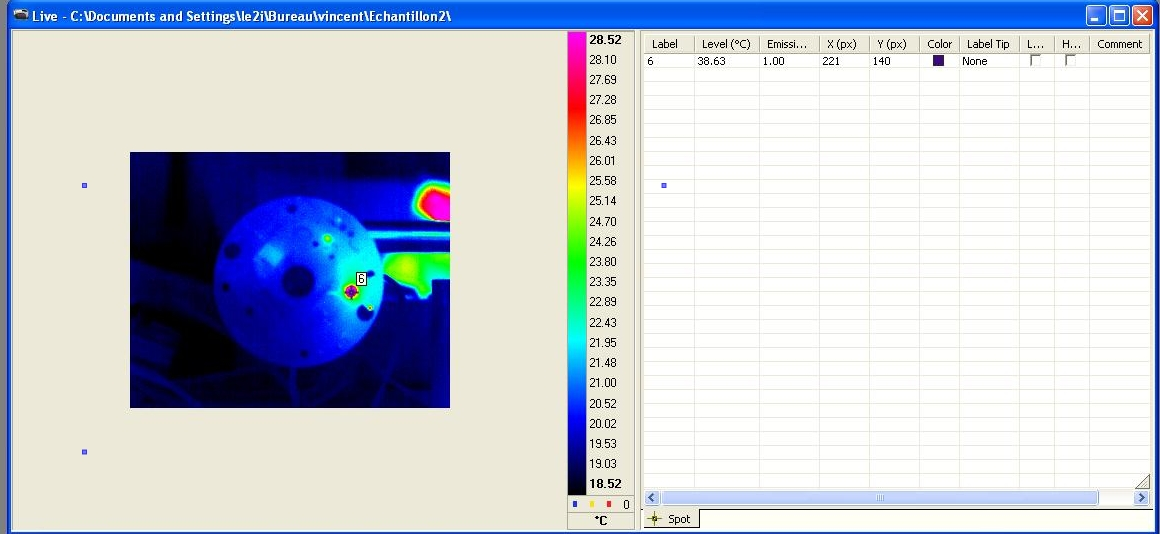
\includegraphics[width=1\linewidth]{Pictures/position1.JPG}
	\caption{The IR image of the circuit with power on}
	\label{fig:two}
\end{figure}
In Figure \ref{fig:two} we see that at position (221, 140) in the view of the camera, the temperature is rising.
We see that the camera measures approximately $39 \textdegree$C.
This value, of course, is not precise because the camera assumes the emissivity of the object to be 1 when, in fact, no real object has emissivity of 1.\\
With this kind of system, we can measure the mean estimated temperature of the whole circuit, as seen in the image below, where we specify the area of interest for the measurement.\\
\begin{figure}[H]
	\centering
	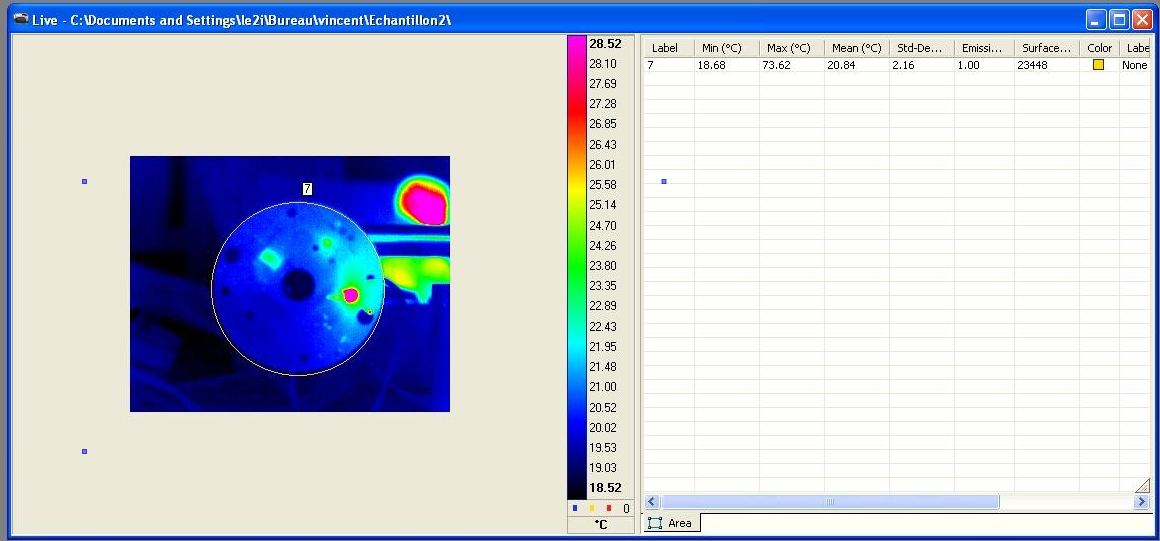
\includegraphics[width=1\linewidth]{Pictures/max1.JPG}
	\caption{Mean temperature measurement of the circuit}
	\label{fig:three}
\end{figure}
Here we can see that the camera estimates the mean temperature of the circuit area to be around $21 \textdegree$C.\\
Another useful measurement that can be done is finding a profile of the temperature along a line on the circuit\\
\begin{figure}[H]
	\centering
	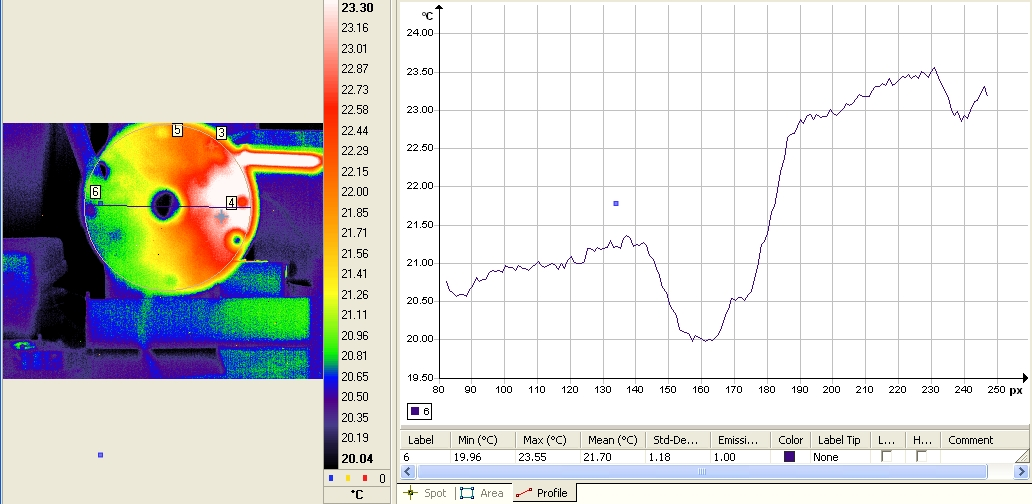
\includegraphics[width=1\linewidth]{Pictures/profile.jpg}
	\caption{Temperature profile of the circuit}
	\label{fig}
\end{figure}


\subsection{Camera Calibration}
\begin{figure}[H]
	\centering
	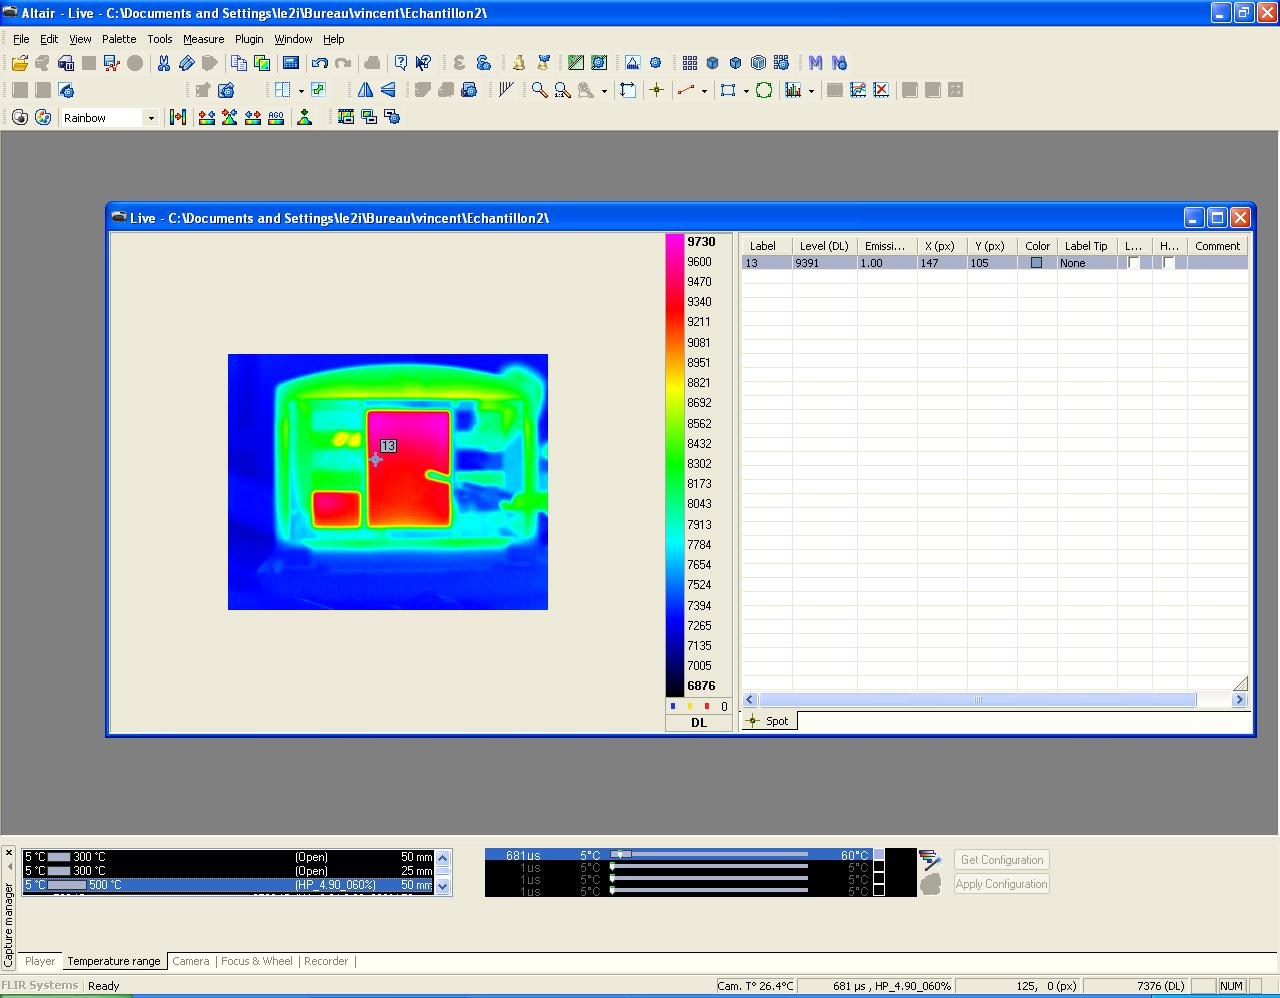
\includegraphics[width=1\linewidth]{Pictures/calib.JPG}
	\caption{Measurement of digital level of a point on a heating plate}
	\label{fig:four}
\end{figure}
As already mentioned, with an infrared camera we cannot precisely measure the temperature of an object without having any information about the properties of the object.
However, we can measure the digital level of an object, knowing that the digital level has to be linearly dependent on the real temperature of the object.
To find the correlation between the digital level and the temperature is to calibrate the temperature measurement of the camera.\\
To find the curve of correlation we measured the digital level and temperature of the same point using an infrared camera as well as an electronic probe, while the temperature of the object was declining.
The resulting curve can be seen below.\\

\begin{figure}[H]
	\centering
	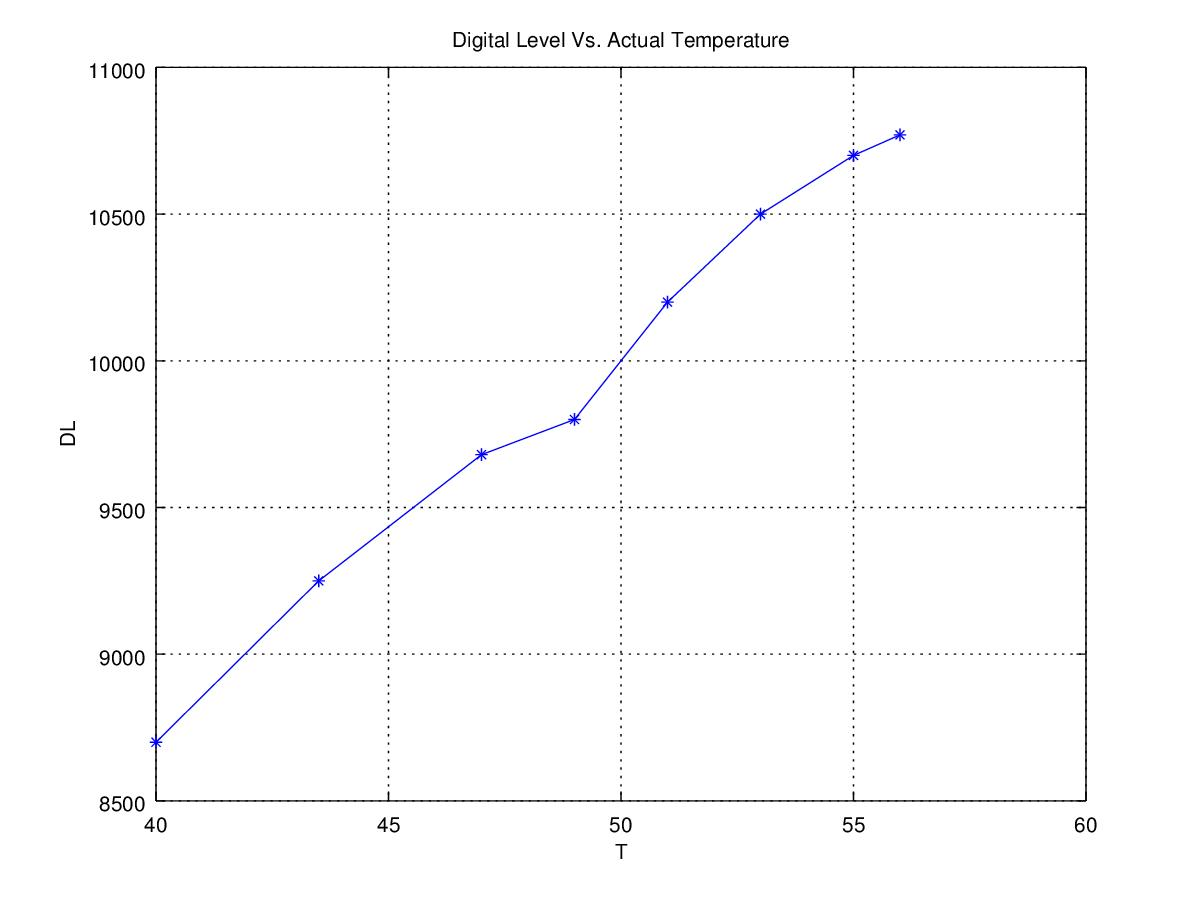
\includegraphics[width=1\linewidth]{Pictures/calibplot.jpg}
	\caption{Calibration curve of the temperature measurement with an infrared camera}
	\label{fig:five}
\end{figure}

We can see that the relationship is linear, except for some errors of measurement.
From the curve we can approximate the real temperature of the object if we have its corresponding digital level, by translating digital level to temperature.
This kind of calibration is not very precise, because the point of measurement has to be the same, as different locations on an object may have different emissivity values.
Another source of error can be the digital probe used for the measurement: it may give incorrect values for the temperature depending on the duration of the measurement, the temperature of the environment, etc.
All these factors make the measurement inaccurate.
Therefore, the calibration too is inaccurate.
\section{Estimation of Emissivity}
In this section we used a C.A 1875 training bench to estimate the emissivity of different materials.
When the bench is still turned off, its infrared image looks as in the picture below.\\
% training bench cold picture
From the picture we see that the materials with smooth polished surfaces are acting like mirrors: they reflect the infrared rays that fall onto them.\\
Then we turned the bench on.
As the plates heated, the polished surfaces still reflected the heat like mirrors.
The rough areas however, started to change color.
And depending on the type of material in the area, the colors in the infrared image varied.
But we know that the temperature of all the plates is, in fact, the same($55\textdegree$C).
The color difference in the infrared is because of the different emissivity values of the materials.\\
\begin{figure}[H]
	\centering
	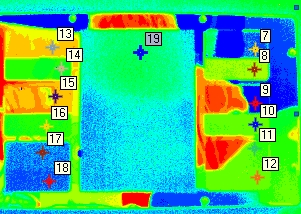
\includegraphics[width=0.6\linewidth]{Pictures/emiss.jpg}
	\caption{Measuring radiance of the materials on the hot plate}
	\label{fig:six}
\end{figure}
As we know emissivity of the surface of a material is its effectiveness in emitting energy as thermal radiation.
It is equal to the ratio of the radiance of the object and the radiance of a black body. And emissivity of a black body is equal to 1.\\
\begin{center}
$\epsilon = \frac{L_{obj}}{L_{bb}} $
\end{center}
So to find the emissivity $L_{obj}$ of the materials on the hot plate, first we measured the radiance of the materials using the Altair software. 
Then using the given emissivity of the black plate as reference, we calculate emissivity to find its value for all materials:\\
\begin{center}
$\epsilon = \frac{L_{obj}}{L_{bb}} $ and $\epsilon_{0} = \frac{L_{0}}{L_{bb}} $,
\end{center}
where $\epsilon_{0}$ is the emissivity of the black plate and is 0.95. $L_{0}$ is the radiance of the black plate and is measured along with all other materials.\\
From the two formulas above we have\\
\begin{center}
$\frac{\epsilon}{\epsilon_{0}} = \frac{L_{obj}}{L_{0}} $ ,
\end{center}
And finally,\\
\begin{center}
$\epsilon = \epsilon_{0} \frac{L_{obj}}{L_{0}} $

\end{center}
Using this relationship, we calculate the emissivity for all materials. 
The results are presented in the table below.\\
\\
\begin{center}
\begin{tabular}{|c|c|c|}
\hline 
 & Radiance(w/$m^{2}$/sr) & Emissivity\tabularnewline
\hline 
\hline 
Polish steel & 2.42 & 0.74\tabularnewline
\hline 
Stainless steel & 1.88 & 0.58\tabularnewline
\hline 
Laminate & 2.40 & 0.74\tabularnewline
\hline 
Red copper & 1.50 & 0.46\tabularnewline
\hline 
Brass & 1.61 & 0.49\tabularnewline
\hline 
Aluminium & 1.36 & 0.42\tabularnewline
\hline 
Black plate & 3.10 & 0.95\tabularnewline
\hline 
\end{tabular}
\end{center}

\section{Transmission and reflection coefficients}
\subsection{Transmission coefficients}
In this part, we first measure the temperature in a certain point in a object, which is Songyou's hand, and snap the picture, which is Figure \ref{fig:transa}.
We then snap two more pictures when covering glass and PVC  camera, respectively (Figure \ref{fig:transb}, Figure \ref{fig:transc}) .\\
\\
According to the Figure \ref{fig:Transf}, we can easily get the transmission coefficient as below:
$$
t_{glass} = \frac{21.70}{32.86} = 0.6604
$$
$$
t_{PVC} = \frac{24.73}{32.86} = 0.7526
$$
\subsection{Reflection coefficients}
For the sake of measuring reflection coefficient of copper, we first set a point in an object (finger), and snap the corresponding infrared image.
And then we snap another image of the copper-reflected finger.
They are shown in Figure \ref{fig:finger}. 
Based on the temperature measured by camera, we can get the reflection coefficient of copper.
$$
r_{copper} = \frac{31.12}{33.72} = 0.9229
$$
\begin{figure}[H]
	\centering
	\subfigure[Original]{\label{fig:transa}
	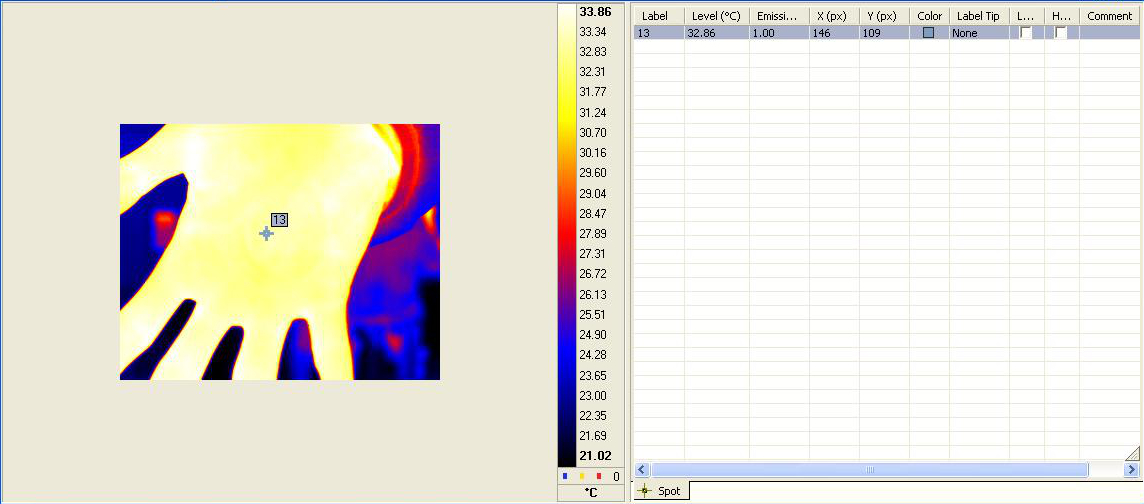
\includegraphics[width=\linewidth]{Pictures/Transf.jpg}
	}
	\subfigure[Glass]{\label{fig:transb}
	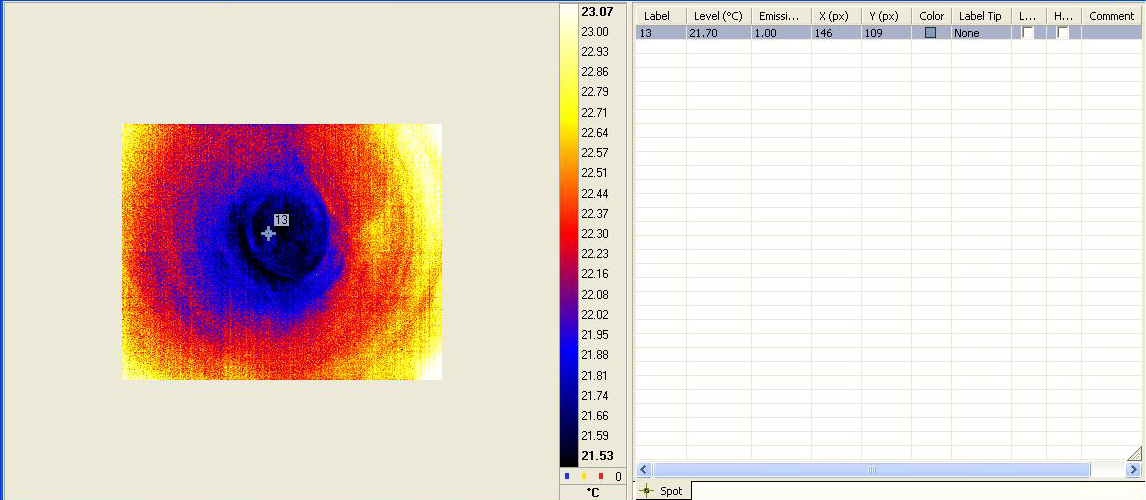
\includegraphics[width=\linewidth]{Pictures/Transf_glass.jpg}
	}
	\subfigure[PVC]{\label{fig:transc}
	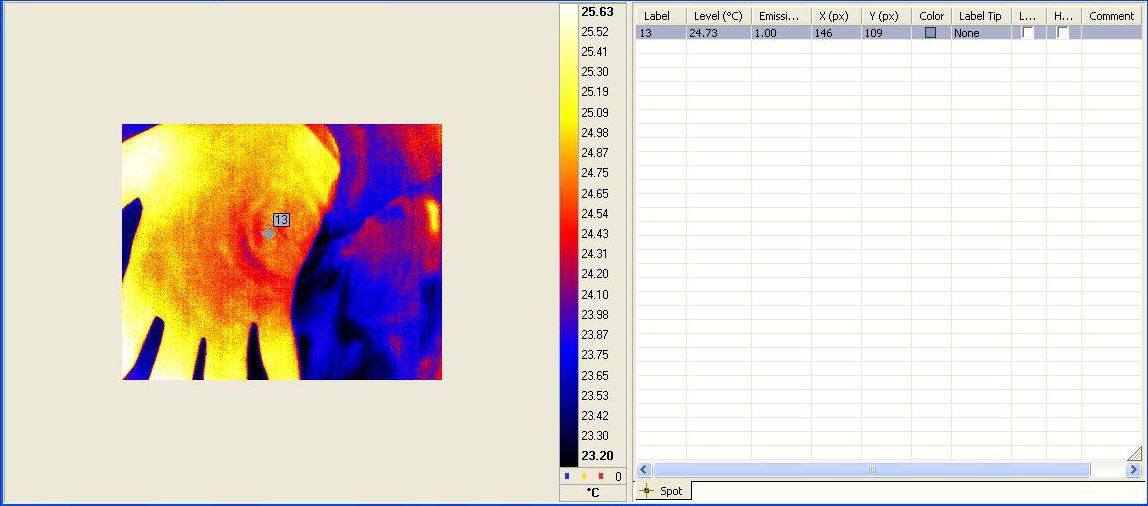
\includegraphics[width=\linewidth]{Pictures/Transf_pvc.jpg}
	}
	\caption{Infrared images of hand}
	\label{fig:Transf}
\end{figure}

\begin{figure}[H]
	\centering
	\subfigure[Original]{\label{fig:fina}
	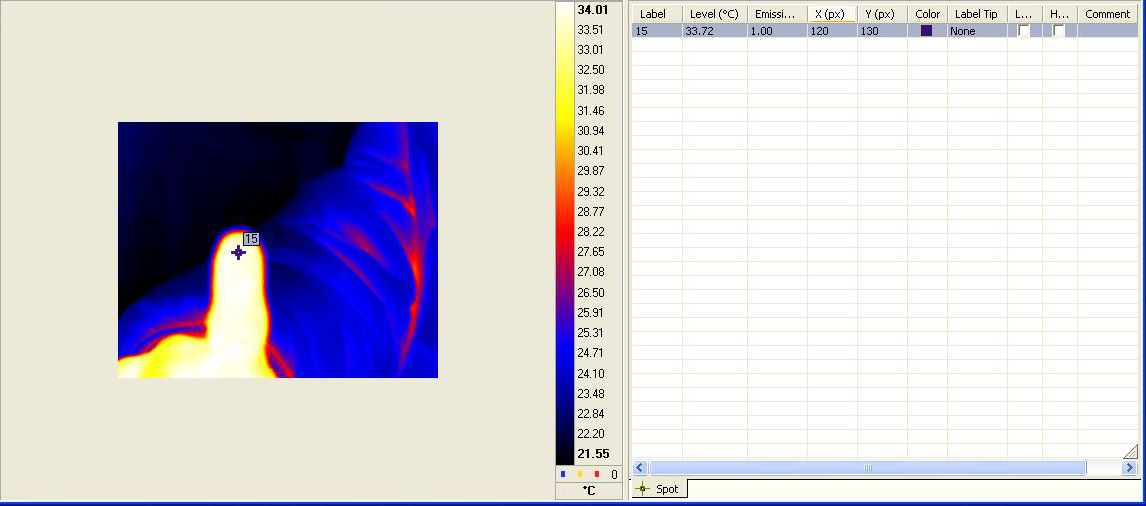
\includegraphics[width=\linewidth]{Pictures/finger2.jpg}
	}
	\subfigure[Copper-reflect finger]
	{\label{fig:finb}
	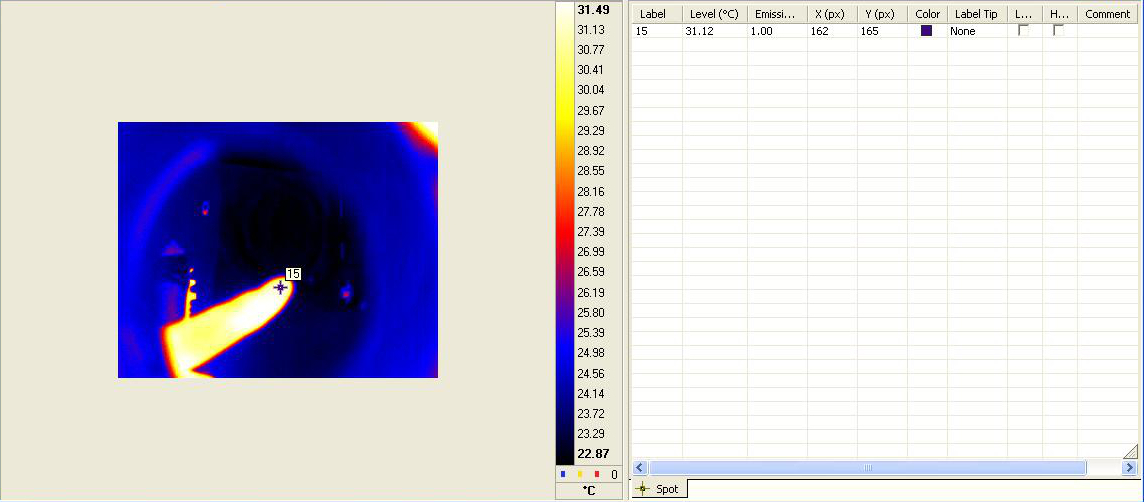
\includegraphics[width=\linewidth]{Pictures/finger.jpg}
	}
	\caption{Infrared images of finger}
	\label{fig:finger}
\end{figure}


\section{Active thermography (Second experiment)}

In this experiment, we use a plate with some holes to see the temperature difference in the plate and holes.
First we will fix the frequency of voltage generator to 1$Hz$ in order to avoid unnecessary external disturbance.
Before we open IR source, which is a halogen, the infrared image is shown in Figure \ref{fig:holea}.
We cannot see the holes from the images first. 

\begin{figure}[H]
	\centering
	\subfigure[Before]{\label{fig:holea}
	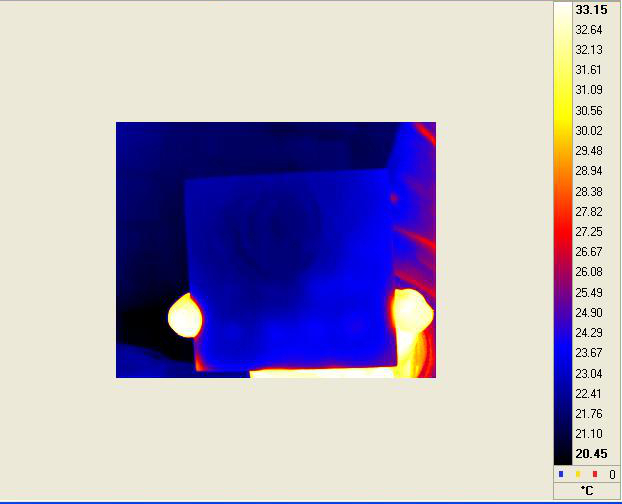
\includegraphics[width=0.4\linewidth]{Pictures/holes_cropped.jpg}
	}
	\subfigure[After]{\label{fig:holeb}
	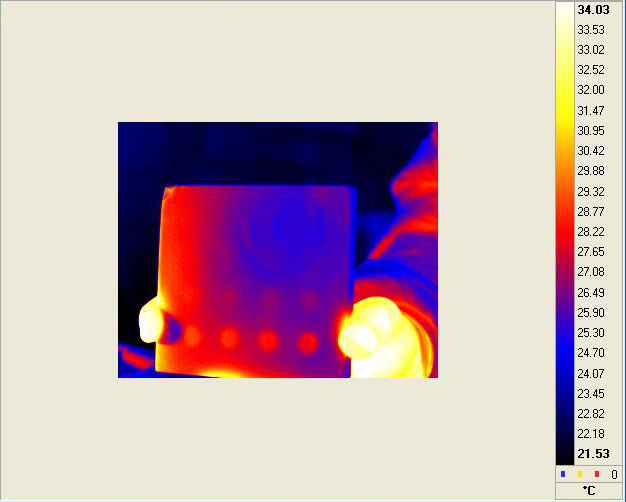
\includegraphics[width=0.403\linewidth]{Pictures/holes2_cropped.jpg}
	}
	\caption{Before and after turning on halogen}
	\label{fig:hole}
\end{figure}

When we turn on the hologen light, the infrared image is shown in Figure \ref{fig:holeb}. We can easily see the holes and tell that the hole parts have higher temperature than other parts in the plane.

\section{Conclusion}
We learn several main application of thermography in this lab. First we have knowledge about how to calibrate infrared camera. This is an essential job because only after calibration can we acquire correct images. Second, we study how to measure emissivity coefficient of different metal, reflection of copper and transmission coefficient of glass and PVC. Third, we also have a chance to see different thickness of same material will lead to different temperatures.

\section{References}
{[}1{]} - C.A 1875, Thermography training bench. http://www.chauvin-arnoux.com/sites/default/files/D00HDX78\
_4.PDF\\
{[}2{]} - Tehnical Support. Emissivity in the Infrared. http://www.optotherm.com/emiss-effects.htm\\
{[}3{]} - Emissivity. https://en.wikipedia.org/wiki/Emissivity


\end{document}